%!TEX root = diploma.tex
% Добавьте ссылку на файлы с текстом работы
% Можно использовать команды:
%   \input или \include
% Пример:
%    \input{mainfiles/1-section} или \include{mainfiles/2-section}
% Команда \input позволяет включить текст файла без дополнительной обработки
% Команда \include при включении файла добавляет до него и после него команду
% перехода на новую страницу. Кроме того, она позволяет компилировать каждый файл
% в отдельности, что ускоряет сборку проекта.
% ВАЖНО: команда \include не поддерживает включение файлов, в которых уже содержится команда \include,
% т.е. не возможен рекурсивный вызов \include
\newcommand*{\Source}{
    %\include{mainfiles/0-annotation}
    %!TEX root = ../diploma.tex
\section{Введение} 

В последние годы нейронные сети (НС) приобрели большую популярность в
применениях машинного обучения к различным прикладным задачам. Отчасти это
обусловлено приростом вычислительных мощностей графических процессоров (ГП):
современные НС часто обучают и запускают с использованием нескольких ГП,
вычисления происходят на облачных серверах и кластерах.

В приложениях на мобильных устройствах с использованием НС иногда возникает
потребность вычисления предсказаний НС непосредственно на самих мобильных
устройствах. Причин этому несколько, в частности: защита данных пользователя,
возможность использования приложения без доступа к сети Интернет, сокращение
затрат на сервера, уменьшение временной задержки на получение предсказания НС. 

Вместо использования центрального процессора мобильного устройства для
вычисления предсказаний НС более эффективно вычисление на его ГП, поскольку
многие операции в НС можно разбить на множество маленьких задач, решаемых
независимо друг от друга, что вполне соответствует архитектурным особенностям
ГП.  

При решении задач, связанных с классификацией и обработкой изображений и
видеопоследовательностей, активно используются разновидности идеи сверточных
нейронных сетей (СНС), предложенной в работе~\cite{cnn}. Также СНС оказались
эффективными и в решении задач из области обработки естественного
языка~\cite{conv_nlp},~\cite{cnn_text_class}. На примере сети
ResNeXt~\cite{resnext} было показано, что архитектурная реализация сверточных
слоев в СНС с помощью групповых сверток, изначально предложенных в
работе~\cite{alexnet}, улучшает точность предсказания, а также вычислительно
более эффективна по сравнению с классическими свертками.

Операции двумерной свертки в СНС вычислительно затратны и возникает естественное
желание добиться эффективности их вычисления. Для их ускорения при фиксированном
размере ядра используются вариации алгоритма вычисления сверток
Винограда~\cite{winograd1980arithmetic} — это позволяет ускорить вычисление
операции свертки в несколько раз.

В силу ограниченности ресурсов мобильного устройства также есть проблемы
потребления памяти и электрической энергии. Особенности обращений в память ГП
влияют на время их выполнения, что тоже сказывается на временных затратах.

Основной вклад данной работы заключается в следующем:
\begin{itemize}
    \item разработан метод оптимизации, позволяющий сокращать объем используемой
    памяти и общее время исполнения;
    \item предложенный метод реализован в программно-аппаратной части библиотеки
    искусственного интеллекта MindSpore Lite\footnote{Кодовая база
    \texttt{MindSpore}: \url{https://github.com/mindspore-ai/mindspore}.} на
    языке C++ с использованием интерфейса прикладного программирования Vulkan;
    \item произведено эмпирическое исследование предложенного метода и его
    сравнение с базовой реализацией и подходами из
    работ~\cite{pisarchyk2020efficient},~\cite{node_level_par}.
\end{itemize}

Настоящая работа организована следующим образом. В разделе~\ref{sec:task}
формально описываются задача оптимизации памяти и задача параллельных
вычислений. Обзор существующих подходов к их решению приводится в
разделе~\ref{sec:literature}. В разделе~\ref{sec:method} описывается
предложенный метод. Экспериментальное исследование метода и сравнение с другими
подходами приводится в разделе~\ref{sec:exp}.

    %!TEX root = ../diploma.tex
\section{Постановка задачи}\label{sec:task}

Пусть $\mathbb{R}$ — множество вещественных чисел, будем называть
\textit{тензорами} многомерные массивы с элементами из $\mathbb{R}$, $\mathbb T
= \bigcup\limits_{n=1}^{\infty}\bigcup\limits_{\mathbb{T}_1,\ldots,\mathbb{T}_n
\in \left\{\mathbb{R}^{s} \mid s \in \mathbb{N}^{+}\right\}} \mathbb{T}_1 \times
\cdots \times \mathbb{T}_n$ — множество всевозможных кортежей из тензоров.

\Def{\emph{Ациклическим графом вычислений (АГВ)} назовем тройку $\langle G(V,
E), \mathbf{op}, \mathbf{t}\rangle$, где $G(V, E)$ — ориентированный
ациклический граф, в котором:
\begin{itemize}
    \item $\mathbf{op}: V \rightarrow (\mathbb T \rightarrow \mathbb T)$ —
    сопоставление вершинам операций, которые отображают набор входящих в вершину
    тензоров в набор выходящих.
    \item $\mathbf{t}: E \rightarrow \bigcup\limits_{s\in \mathbb{N}^{+}}
    \mathbb{R}^{s}$ — каждому ребру соответствует некоторый тензор, причем
    разные ребра могут соответствовать одному и тому же тензору тогда и только
    тогда, когда эти ребра исходят из одной вершины. \end{itemize}}

Вычисление предсказаний НС можно представить в виде АГВ, пример такого
представления приведен на Рис.~\ref{fig:cfg}. Данная работа сфокусирована на
улучшении программно-аппаратной части вычисления предсказаний НС, без
рассмотрения оптимизации архитектуры самой НС или процесса ее обучения. Целью
работы является исследование существующих методов оптимизации объема
используемой памяти и затраченного времени на вычисление предсказания НС на
уровне АГВ, а также разработка и реализация метода, позволяющего одновременно
оптимизировать и затраченное время, и объем используемой памяти.

\begin{figure}[h]
\centering
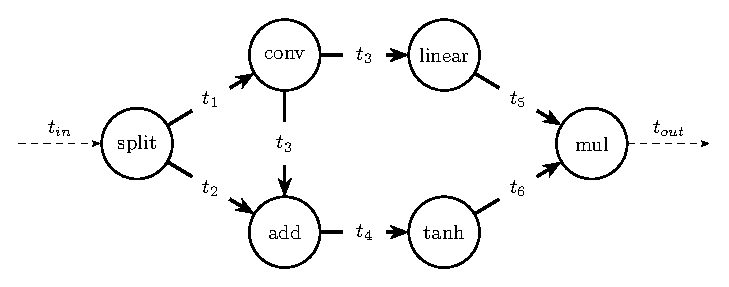
\includegraphics[scale=1.05]{dag.pdf}
\caption{Пример ациклического графа вычислений}
\label{fig:cfg}
Пунктирными линиями изображены входной и выходной тензор, которые присутствуют в
вычислениях, но отсутствуют в самом графе.
\end{figure}

\subsection{Задача оптимизации памяти}

Параметры НС, представляющие собой тензоры, можно разделить на четыре категории:
\begin{itemize}
    \item Константные, так же веса НС
    \item Входные — то, что подается на вход НС
    \item Выходные — предсказание НС
    \item Промежуточные — не относящиеся к трем остальным категориям
\end{itemize}
Входные и константные тензоры копируются из оперативной памяти в память ГП перед
вычислением сети, выходные — копируются из памяти ГП в оперативную память после
произведенных вычислений. Для промежуточных же тензоров память может быть
использована повторно, если это не нарушает корректности производимых
вычислений.

В настоящей работе мы рассматриваем задачу предварительного распределения
памяти, то есть размеры промежуточных тензоров НС заранее известны. Выделение
блока памяти производится указанием для промежуточных тензоров сдвигов на
соответствующие им ячейки памяти, начиная с которых тензоры могут быть записаны
или считаны, располагаясь как непрерывные блоки. Выбор такого подхода работы с
памятью обусловлен тем, что интерфейс прикладного программирования Vulkan,
используемый для реализации программно-аппаратной части MindSpore Lite,
предполагает резервирование приложением продолжительно используемой памяти,
которую он может самостоятельно использовать.

Для соблюдения корректности результата последовательное вычисление НС необходимо
производить в порядке любой топологической сортировки АГВ (ТС), т.е. для
вычисления в данный момент некоторой операции необходимо и достаточно, чтобы все
входные тензоры были вычислены.

\noindent\textbf{Формулировка задачи оптимального распределения памяти}

Обозначим множество тензоров, соответствующих ребрам в АГВ $\langle G(V, E),
\mathbf{op}, \mathbf{t}\rangle$, как ${T} = \text{im}(\mathbf{t}) =
\left\{\mathbf{t}(e_1), \ldots, \mathbf{t}(e_{|E|})\right\}$. Для тензора
$t\in{T}$ обозначим размер тензора, который он занимает в памяти, как
$w_t\in\mathbb{N}$. Тогда задачу распределения памяти можно задать в виде
следующей задачи оптимизации:
\begin{subequations}\label{eqn:opt}
    \renewcommand{\theequation}{\theparentequation\asbuk{equation}}
\begin{align}[left ={\empheqlbrace}]
    & \max\limits_{t\in {T}}(x_t+w_t) \rightarrow \min & \label{minmax} \\
    & x_{t_1} + w_{t_1} \le x_{t_2} \vee x_{t_2} + w_{t_2} \le x_{t_1} & \notag
    \\
    & \text{\ }\forall t_1,t_2 \in{T}: \text{$t_1$ и $t_2$ могут использоваться
    одновременно} & \label{cond:intersect} \\
    & x_t \in \mathbb{Z},\,x_t \ge 0 & \forall t\in {T} \label{cond:nonneg}
    \end{align}
\end{subequations}
где $x_t$ — сдвиг в памяти ячейки начала размещения тензора $t$.
Ограничение~\ref{cond:intersect} запрещает тензорам использовать одну и ту же
память, если может возникнуть конфликт, а~\ref{cond:nonneg} отражает то, что
сдвиг в памяти обязан быть целым неотрицательным числом. При этих ограничениях
требуется использовать как можно меньший объем памяти, этому соответствует
выражение~\ref{minmax}.

\subsection{Задача параллельных вычислений}

Вычисление НС с помощью программы представляется в виде конвейера из команд,
которые можно логически разбить на следующие типы:
\begin{enumerate}
    \item Копирование блока из оперативной памяти в память ГП\label{op:copyto}
    \item Копирование блока из памяти ГП в оперативную память\label{op:copyfrom}
    \item Исполнение вычислительного \textit{шейдера} (программы, выполняющейся
    параллельно несколькими блоками потоков ГП)\label{op:shaders}
    \item Барьер памяти вида запись/чтение между операциями типа~\ref{op:copyto}
    и операциями типа ~\ref{op:shaders}.\label{op:bar-copy-comp}
    \item Барьер памяти вида запись/чтение между операциями
    типа~\ref{op:shaders}  и операциями типа
    ~\ref{op:shaders}.\label{op:bar-comp-comp}
    \item Барьер памяти вида запись/чтение между операциями
    типа~\ref{op:shaders}  и операциями типа
    ~\ref{op:copyfrom}.\label{op:bar-comp-copy}
\end{enumerate}

Перед началом интересующих нас вычислений выполняются команды
типов~\ref{op:copyto} и~\ref{op:bar-copy-comp}, после —~\ref{op:bar-comp-copy}
и~\ref{op:copyfrom}. Операции (вершины в АГВ) суть один или несколько
вычислительных шейдеров, их вычисление относится к типу команд~\ref{op:shaders},
а между вычислением вершин размещаются при необходимости барьеры
памяти~\ref{op:bar-comp-comp}.

Под \textit{базовой программной реализацией} вычислений НС с помощью ГП будем
подразумевать следующее: вычисление операций происходит в порядке произвольной
топологической сортировки АГВ; между каждой последовательной парой операций в
конвейере располагается барьер памяти; для каждого тензора выделяется отдельный
блок памяти, непересекающийся ни в какой момент времени с остальными.

\begin{figure}
\centering
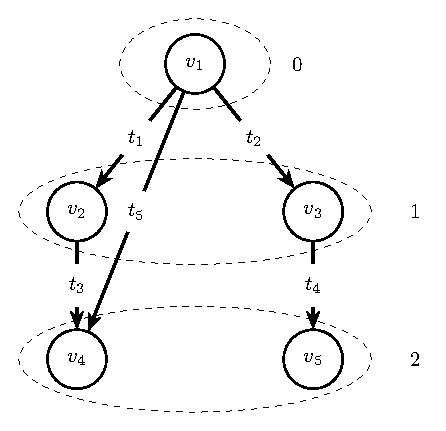
\includegraphics[scale=1.2]{par.pdf}
\caption{Пример АГВ, в котором возможно параллельное вычисление некоторых вершин}
\label{parcfg}
Пунктирными линиями обведены подмножества\\ независящих друг от друга вершин
\end{figure}

При такой реализации возникает проблема избыточных синхронизаций, вызывающих
простои в вычислениях. Сократить время простоев возможно, разбив АГВ на
несколько блоков так, что внутри каждого блока вершины будут попарно
\textit{независимы} (не существует пути из одной в другую), и можно выбрать
порядок вычисления этих блоков, при котором все зависимости будут соблюдаться
(аналогично топологической сортировке вершин). Пример такого разбиения приведен
на Рис.~\ref{parcfg}.

Задача параллельных вычислений состоит в том, чтобы найти эффективный способ
получать разбиение АГВ на непересекающиеся подмножества попарно независимых
вершин так, чтобы не было циклической зависимости этих подмножеств друг от
друга. Также нужно исследовать применимость способа на практике.

    %!TEX root = ../diploma.tex

\section{Обзор литературы}\label{sec:literature}
\subsection{Задача оптимизации памяти}

На Рис.~\ref{fig:cfg} приведен пример АГВ: можно заметить, что, например,
выделенные блоки памяти для следующих пар тензоров:
\begin{itemize}[nosep]
    \item $(t_2,t_3),(t_5,t_6)$ — не могут пересекаться независимо от выбора ТС
    \item $(t_1,t_4),(t_1,t_5),(t_3,t_6)$ — могут пересекаться независимо от
    выбора ТС
    \item $(t_2,t_4),(t_4,t_6)$ — могут пересекаться, если размерности
    соответствующих входов и выходов совпадают для операций \textbf{add} и
    \textbf{tanh}, поскольку они являются поэлементными операциями
    \item $(t_3,t_4)$ — могут или не могут пересекаться в зависимости от ТС
    (необходимо ли хранить значение $t_3$ после вычисления операции
    \textbf{add}) и совпадения размерностей $t_3$ и $t_4$
\end{itemize}
На Рис.~\ref{fig:ints} для этого примера приведена одна из возможных
топологических сортировок и помечены времена жизни для тензоров.

\begin{figure}[ht]
\centering
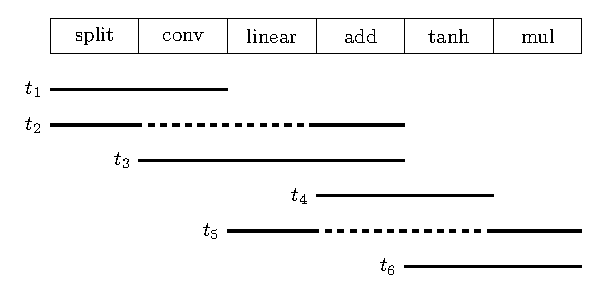
\includegraphics[scale=1.1]{ints}
\caption{Время жизни тензоров}
\label{fig:ints}
\end{figure}


Задача~\ref{eqn:opt} является NP-полной в случае различных размеров тензоров и
сводится, например, к задаче 3-разбиений~\cite{np_complete}. Тем не менее
возможен поиск приближенного решения эвристическими
алгоритмами~\cite{sekiyama2018profile},~\cite{pisarchyk2020efficient}.

В работе~\cite{sekiyama2018profile} задача~\ref{eqn:opt} выражается как частный
случай задачи упаковки прямоугольников (разместить прямоугольники в контейнер с
заданной шириной и наименьшей высотой), решаемый эвристическим алгоритмом. В
работе~\cite{pisarchyk2020efficient} для каждого тензора $t$ АГВ вычисляется
кратчайший отрезок вершин, включающий в себя все вершины, для которых $t$
является входящим или выходящим ребром (назовем его \textit{временем жизни}
$t$); тензорам $t_1$ и $t_2$ разрешено использовать общую память тогда и только
тогда, когда пересечение их времен жизни пусто. Далее описывается жадный
алгоритм, в котором перебираются тензоры по убыванию их размера, и для каждого
производится поиск наименьшего зазора в памяти, вмещающего его. Экспериментально
показывается, что описанная ими стратегия достигает результатов не хуже (иногда
лучше), чем эвристический метод из~\cite{sekiyama2018profile}, на примере
нескольких НС.

\subsection{Задача параллельных вычислений}
\label{subsec:literature:parallel}

Для разбиения множества вершин АГВ на непересекающиеся подмножества независимых
вершин можно использовать следующий подход, представляющий собой динамическое
программирование на ациклическом графе (предложен, например,
в~\cite{node_level_par}):
\begin{enumerate}
    \item Рассмотрим вершины графа в порядке топологической сортировки:
        \begin{itemize}
            \item если у очередной вершины $v$ нет входящих ребер,
            инициализируем $\variablename{maxdist}(v) = 0$;
            \item иначе, находим у вершины $v$ предка $w$ с наибольшим значением
            $\variablename{maxdist}(w)$, и затем инициализируем
            $\variablename{maxdist}(v) = \variablename{maxdist}(w)+1$.
        \end{itemize}
    \item Пусть $D=\max\limits_{v \in V}\variablename{maxdist}(v)$. Построим для
    вершин $V$ разбиение на подмножества: $\left\{L_0,\ldots,L_D\right\}$, где
    $L_i = \{v \mid \variablename{maxdist}(v) = i\}.$
\end{enumerate}
Будем называть $L_i, i\in\overline{0,D}$ слоями АГВ. Очевидно, $\forall
i,j\in\overline{0,D}\ i\not=j \rightarrow L_i \cap L_j = \emptyset$. Покажем,
что в каждом множестве находятся только попарно независимые вершины.

\newtheorem{statement}{Утверждение}
\numberwithin{statement}{section}
\begin{statement}
    \label{statement:maxdist}
    $\forall i\in\overline{0,D}\ \forall v,u \in L_i\ v$ и $u$ — независимы.
\end{statement}
\begin{proof}
    Допустим, что $v$ и $u$ не являются независимыми, то есть существует либо
    путь из $v$ в $u$, либо из $u$ в $v$. Но тогда длина наибольшего пути не
    может совпадать: в первом случае $\variablename{maxdist}(v) <
    \variablename{maxdist}(u)$, во втором $\variablename{maxdist}(u) <
    \variablename{maxdist}(v)$. Следовательно, если $v$ и $u$ принадлежат одному
    и тому же слою, то они независимы.
\end{proof}

Такой способ не гарантирует нахождения наибольших групп независимых вершин,
однако является вычислительно эффективным и для представлений НС в виде АГВ
находит приемлемое решение, что показано в разделе~\ref{sec:exp}.

    %!TEX root = ../diploma.tex

\section{Предложенный метод}\label{sec:method}

Предлагается для начала рассмотреть нижеизложенный способ, позволяющий
объединить эвристический метод оптимизации для задачи памяти, изложенный в
работе~\cite{pisarchyk2020efficient}, с описанным в
подразделе~\ref{subsec:literature:parallel} подходом разбиения АГВ на слои
независимых вершин для сокращения затрат на синхронизацию (в частности,
параллельное вычисление вершин).

Введем предикат $F: T\times T \rightarrow \{0,1\}$:
$$F(t_1, t_2) =
\begin{cases}
1, &\text{найдется слой, одновременно использующий $t_1$ и $t_2$}\\
0, &\text{иначе} \end{cases}$$ Использовав его, как дополнительное ограничение
при проверке пересечения времен жизни тензоров, можно сформулировать приведенный
алгоритм~\ref{alg:euristic_search}. Для выполнения алгоритма требуется
предварительно найти времена жизни для всех тензоров, за это отвечает
алгоритм~\ref{alg:lifespans}.

При введении дополнительных ограничений может оказаться, что объем потребляемой
памяти возрастает по сравнению с изначальным алгоритмом. Помимо этого имеется
фактор среднего времени доступа в память ГП (чтение/запись), на который может
влиять кэширование блоков памяти.

С целью варьирования дополнительных ограничений на тензоры, которые не могут
использовать общую память, и количества точек синхронизации, предлагается
дополнительно разбивать каждый слой АГВ на несколько непересекающихся
\textit{групп} одинакового размера (кроме, возможно, последней). Тогда
вычисление отдельно взятого слоя будет представлять собой последовательное
вычисление нескольких групп, между которыми будут установлены дополнительные
точки синхронизации. Новые ограничения на совместное использование памяти
тензорами зададим следующим образом:
\begin{gather*}
    F(t_1, t_2) = \begin{cases}
    1, &\text{найдется группа, одновременно использующая $t_1$ и $t_2$}\\
    0, &\text{иначе} \end{cases}
\end{gather*}

Таким же образом полученный предикат $F(\cdot, \cdot)$ можно использовать в
алгоритме~\ref{alg:euristic_search}.

\begin{figure}
    \centering
    \begin{subfigure}[t]{\textwidth}\centering
    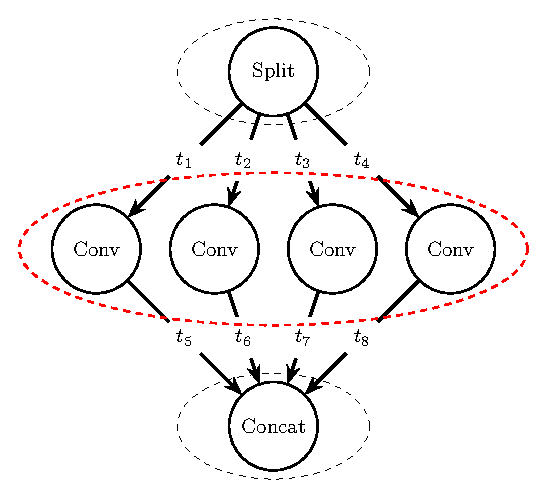
\includegraphics[width=0.6\textwidth]{nogroups}
    \caption{}
    \end{subfigure}
    \begin{subfigure}[t]{\textwidth}\centering
    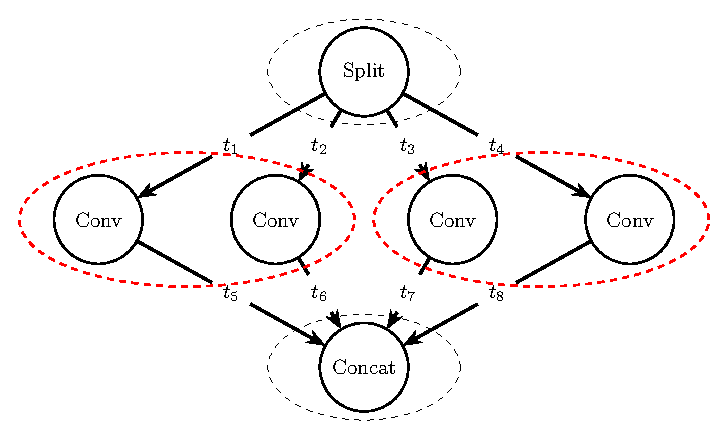
\includegraphics[width=0.8\textwidth]{groups}    
    \caption{}
    \end{subfigure}
    \caption{Пример применения предложенного метода с разбиением на одну группу (а) две группы (б)}
\end{figure}

\begin{algorithm}
    \caption{Нахождение времен жизни тензоров}
    \label{alg:lifespans}
    \begin{algorithmic}[1] % The number tells where the line numbering should start
        \Function{CalculateTensorLifespans}{}
            \State from $\gets\emptyset$ \Comment{ассоциативный массив (тензор, начало времени жизни)}
            \State to $\gets\emptyset$ \Comment{ассоциативный массив (тензор, конец времени жизни)}
            \ForAll{$v_i \in V$ (\textbf{в порядке топологической сортировки})}
                \ForAll{$t$ — входящий/исходящий тензор для $v_i$}
                    \If{$t \notin$ from}
                        \State from($t$) $\gets$ i
                    \EndIf
                    \State to($t$) $\gets$ i
                \EndFor
            \EndFor
            \State lifespan $\gets \left\{[\text{from}(t), \text{to}(t)] \mid t \in T\right\}$
            \State \Return lifespan
        \EndFunction
    \end{algorithmic}
\end{algorithm}

\begin{algorithm}
    \caption{Эвристический поиск распределения памяти}
    \label{alg:euristic_search}
    \begin{algorithmic}[1]
        \Function{CalculateTensorOffsets}{}
            \State lifespan $\gets$ CalculateTensorLifespans()
            \State offset\_records $\gets \emptyset$ \Comment{множество пар (тензор, его сдвиг в памяти)}
            \ForAll{$t$ — промежуточный тензор (\textbf{по убыванию} size($t$))}
                \State prev\_offset $\gets$ 0
                \State best\_offset $\gets$ null
                \State smallest\_gap $\gets \infty$
                \LineComment{пытаемся найти наименьший зазор для $t$}
                \ForAll{(x, offset) $\in$ offset\_records \textbf{по возрастанию} offset}
                    \If{lifespan($t$) $\cap$ lifespan($x$) $\neq \emptyset$ \textbf{или} $F(t, x)=1$}
                        \If{offset $\ge$ prev\_offset}
                            \State gap $\gets$ offset $-$ prev\_offset
                            \If{size$(t)$ $\le$ gap \textbf{и} gap $<$ smallest\_gap}
                                \State smallest\_gap $\gets$ gap
                                \State best\_offset $\gets$ prev\_offset
                            \EndIf
                        \EndIf
                        \State prev\_offset $\gets$ max(prev\_offset, offset + size$(x)$)
                    \EndIf
                \EndFor
                \LineComment{если не нашли зазор, расширяем область памяти}
                \If{best\_offset $=$ null}
                    \State best\_offset $\gets$ prev\_offset
                \EndIf
                \State \textbf{добавляем} (t, best\_offset) \textbf{в} offset\_records
            \EndFor
            \State \Return offset\_records
        \EndFunction
    \end{algorithmic}
\end{algorithm}
\newpage
\noindent\textbf{Планирование запуска АГВ}

При теоретической оценке времени вычисления АГВ будем учитывать следующие
факторы затрат:
\begin{enumerate}
    \item Вычисление вершин/групп вершин
    \item Синхронизации между вычислениями вершин/групп вершин
\end{enumerate}

Время, затраченное на пересылку данных из оперативной памяти в память ГП и
обратно, а также подготовку АГВ к вычислению, учитывать не будем.

Пусть в графе $G=(V,E)$ вершины занумерованы в порядке какой-то топологической
сортировки. Введем обозначения: $\tau(v), v\in V$ — время вычисления вершины
$v$, $s(v_{i}, v_{i+1}), v_{i},v_{i+1}\in V$ — время, затраченное на
синхронизацию между вершинами $v_{i}$ и $v_{i+1}$.

В нашей модели вычислений суммарное затраченное время на вычисление графа $G$
при базовой программной реализации:
$$
\tau(G) = \sum\limits_{i=1}^{n}{\tau(v_i)} + \sum\limits_{i=1}^{n-1}{s(v_{i},v_{i+1})}
$$ 

Используем теперь построенное ранее разбиение на слои для более эффективного
планирования вычислений. Рассмотрим разбиение на слои
$\left\{L_0,\ldots,L_D\right\}$, и для каждого слоя $\tau(L)$ — время вычисления
$L$, $s(L_i, L_{i+1})$ — время, затраченное на синхронизацию между слоями $L_i$
и $L_{i+1}$. Тогда суммарное время вычисления графа $G$:

$$
\tau'(G) = \sum\limits_{i=0}^{D}{\tau(L_i)} + \sum\limits_{i=1}^{D-1}{s(L_{i},L_{i+1})}
$$ 
В таком случае, теоретическое ускорение можно выразить так:
\begin{equation}\label{eqn:speedup}
    S(G) = \frac{\tau(G)}{\tau'(G)} = \frac{\sum\limits_{i=1}^{n}{\tau(v_i)} + \sum\limits_{i=1}^{n-1}{s(v_{i},v_{i+1})}}{\sum\limits_{i=0}^{D}{\tau(L_i)} + \sum\limits_{i=1}^{D-1}{s(L_{i},L_{i+1})}}
\end{equation}
Поскольку при группировке вершин число синхронизаций уменьшается, а в силу роста
степени параллелизма при объединении вершин в группы можно предположить, что
$\tau(L_i) \le \sum\limits_{v\in L_i}\tau(v) \Rightarrow S(G) \ge 1$. В
разделе~\ref{sec:exp} будет протестировано соответствие действительности такой
модели.

    %!TEX root = ../diploma.tex

\section{Результаты экспериментов}\label{sec:exp}

\begin{figure}
\centering
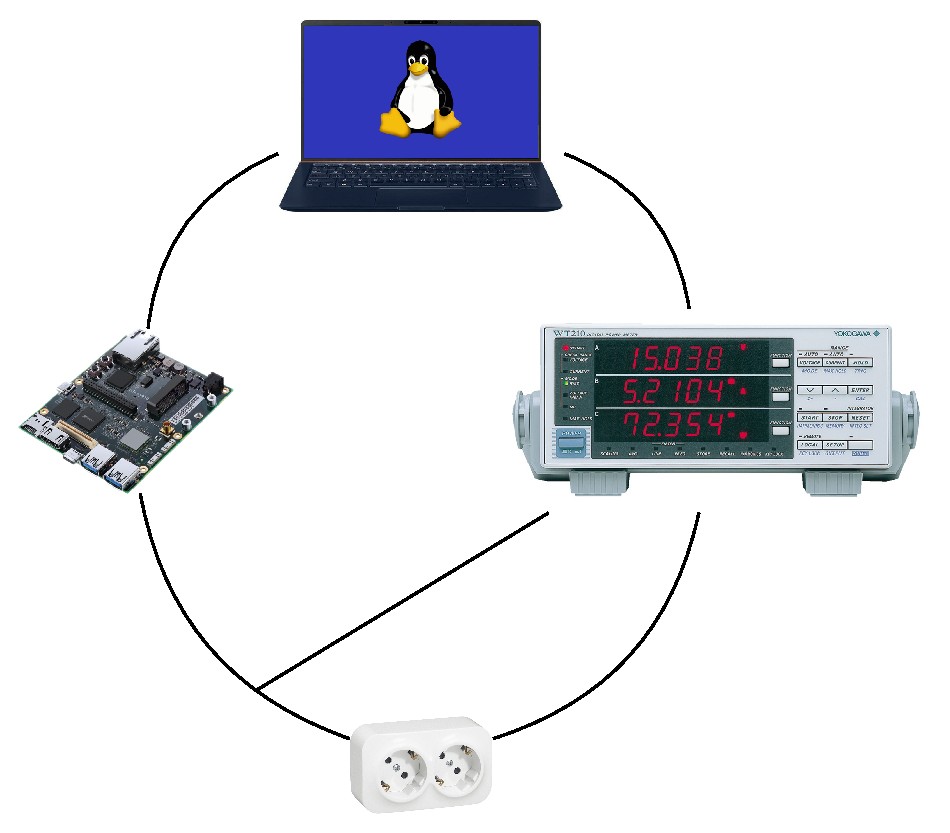
\includegraphics[scale=0.8]{setup}
\caption{Экспериментальная установка}
\label{fig:setup}
\end{figure}

В таблице~\ref{tab:exps} приведены полученные результаты замеров времени и
памяти для некоторых моделей НС: ResNeXt~\cite{resnext},
GoogLeNet~\cite{googlenet}, MobileNetV2~\cite{mobilenetv2},
Xception~\cite{xception}, InceptionV3~\cite{inceptionv3}. При конфигурации
предложенного метода количество групп выбрано одинаковым для всех слоев и
равняется либо 1, либо 2 (поскольку для всех сетей, кроме ResNeXt, размеры
получаемых слоев не превосходят четырех вершин). Из этой таблицы видно, что для
всех НС, кроме ResNeXt, оптимальное потребление памяти (по сравнению с
изначальной эвристикой оптимизации памяти) достигается уже при одной группе, и
разбиение на две группы также не дает улучшения по времени исполнения.

Представляет интерес более тщательный анализ экспериментов для ResNeXt (СНС с
групповыми свертками размера 32). На Рис.~\ref{fig:exp_dispatch_groups}
приведены полученные значения времени исполнения, объема используемой памяти,
числа циклов ожидания обращений в память ГП и среднее потребление электрической
энергии на запуск НС без учета потребления в покое. Оптимальный выбор числа
групп может быть нетривиален: например, исходя исключительно из времени
исполнения, будет оптимально разбить каждый слой на две группы. Если взять также
в расчет потребление памяти и электрической энергии, наилучшим значением может
оказаться 16 или 8 групп. При разбиении на две группы ускорение составляет
6.85\%, а потребление памяти сокращается на 72.4\%.

Полученное сокращение времени вычислений при увеличении числа групп говорит о
том, что модель~\ref{eqn:speedup} оказывается слишком упрощенной. А именно, она
не учитывает, каким образом организован доступ в память ГП ее вычислительными
ядрами. В нашем случае разбиение ResNeXt на две группы вместо одной дает
относительное ускорение на 3.65\%, также сокращается потребление памяти на
2.68\%.

Приведенные измерения производились на плате HiKey970 с мобильным графическим
процессором ARM Mali-G72 MP12, интегрированном в систему на кристалле HiSilicon
Kirin 970. Реализация всех методов и экспериментов произведена в
программно-аппаратной части библиотеки искусственного интеллекта MindSpore Lite
с использованием языка C++ и интерфейса прикладного программирования Vulkan.
Показатели ГП устройства были получены профилированием набором инструментов Arm
Development Studio. Потребление электрической энергии было посчитано при помощи
цифрового измерителя мощности Yokogawa WT210, показания с которого считывались
утилитой командной строки Yokotool\footnote{Исходный код \texttt{Yokotool}:
\url{https://github.com/intel/yoko-tool}.}. Визуально используемая
экспериментальная установка изображена на Рис.~\ref{fig:setup}.

\tabulinesep = 4pt

\begin{table}
    \caption{Результаты экспериментов}
    \label{tab:exps}
    \begin{tabu} to \textwidth{ X[1.6,l] X[1.45,l] *{5}{X[c]}}
        \hline
        Алгоритм & & \tiny{ResNeXt} & \tiny{GoogLeNet} & \tiny{MobileNetV2} &
        \tiny{Xception} & \tiny{InceptionV3}\\
        \thickhline
        \multirow{2}{3cm}{Базовая реализация} & время, мс & 234 ± 5 & 80 ± 3 & 81 ±
        3 & 291 ± 2 & 369 ± 4\\
        & память, Мб & 393.7 & 67.9 & 78.3 & 268.5 & 198.1\\
        \thickhline
        \multirow{2}{3cm}{Оптимизация памяти} & время, мс & 235 ± 6 & 82 ± 1 & 85 ±
        4 & 293 ± 2 & 370 ± 3\\
        & память, Мб & \textbf{108.8} & \textbf{42.4} & \textbf{30.3} &
        \textbf{113.2} & \textbf{122.6}\\ \hline
        \multirow{2}{3cm}{Послойное вычисление} & время, мс & 228 ± 2 & \textbf{77 ±
        1} & \textbf{80 ± 3} & \textbf{290 ± 2} & \textbf{361 ± 3}\\
        & память, Мб & 393.7 & 67.9 & 78.3 & 268.5 & 198.1\\
        \thickhline
        \multirow{2}{3cm}{Разбиение на 1 группу} & время, мс & 227 ± 2 & 78 ± 2 & 82
        ± 3 & \textbf{290 ± 2} & \textbf{361 ± 4}\\
        & память, Мб & 111.8 & \textbf{42.4} & \textbf{30.3} & \textbf{113.2} &
        \textbf{122.6}\\ \hline
        \multirow{2}{3cm}{Разбиение на 2 группы} & время, мс & \textbf{219 ± 2} & 78
        ± 1 & 83 ± 4 & 291 ± 2 & 364 ± 3\\
        & память, Мб & \textbf{108.8} & \textbf{42.4} & \textbf{30.3} & \textbf{113.2} &
        \textbf{122.6}\\ \hline
    \end{tabu}
    \begin{center}
        \item Для результатов замеров времени приведено:\\ среднее значение по
        выборке ± два среднеквадратичных отклонения 
    \end{center}

    \begin{subfigure}[t]{.5\textwidth}
    \centering
    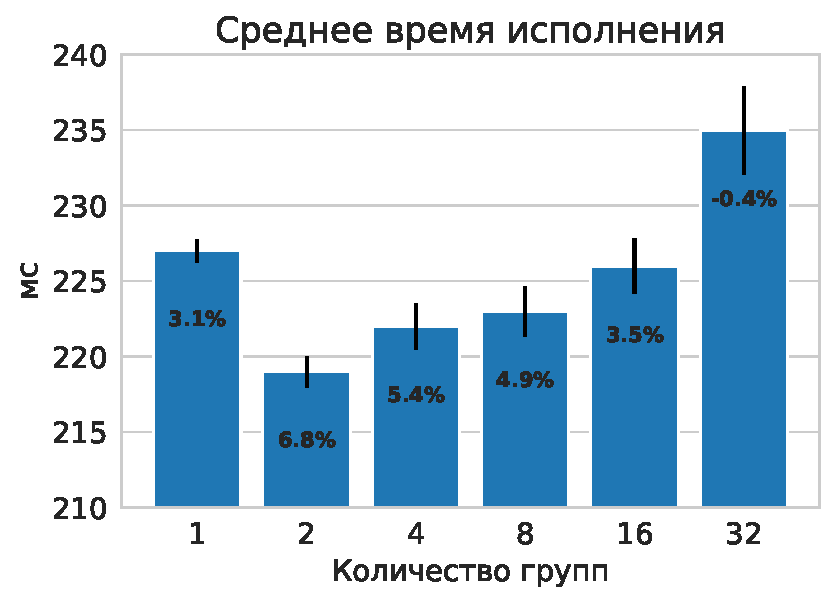
\includegraphics[width=\linewidth]{exp_dispatch_groups.pdf}
    \end{subfigure}
    \hfill
    \begin{subfigure}[t]{.5\textwidth}
    \centering
    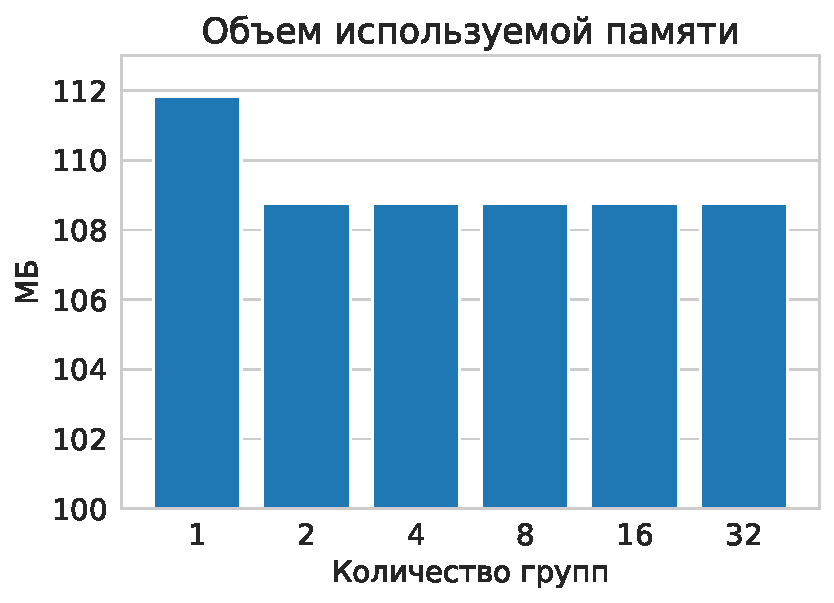
\includegraphics[width=\linewidth]{exp_dispatch_groups_mem.pdf}
    \end{subfigure}
    \begin{subfigure}[t]{.5\textwidth}
    \centering
    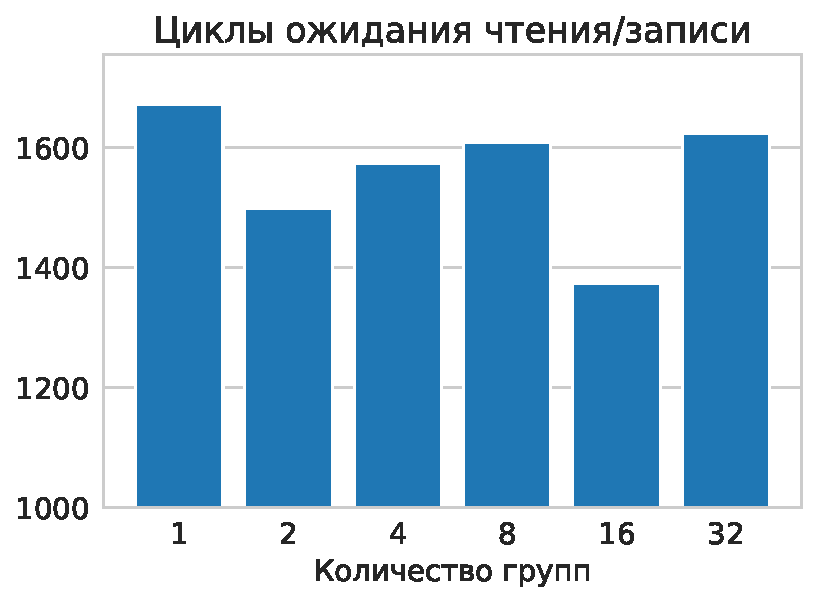
\includegraphics[width=\linewidth]{exp_dispatch_stall.pdf}
    \end{subfigure}
    \hfill
    \begin{subfigure}[t]{.5\textwidth}
    \centering
    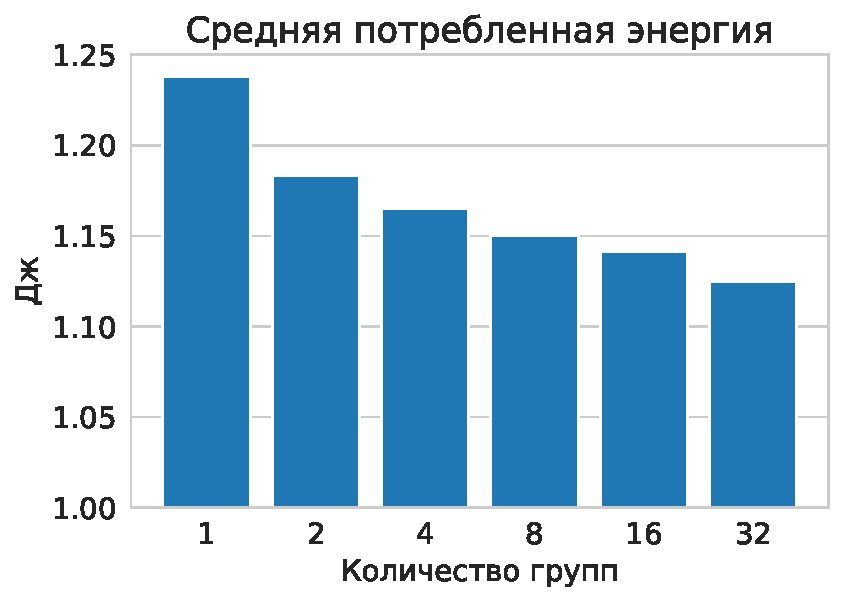
\includegraphics[width=\linewidth]{exp_dispatch_energy.pdf}
    \end{subfigure}
    \captionof{figure}{Столбчатые диаграммы с результатами применения предложенного метода к сети ResNeXt}
    \label{fig:exp_dispatch_groups}
\end{table}

    %!TEX root = ../diploma.tex

\section{Заключение}

В настоящей работе были рассмотрены задача оптимизации используемого объема
памяти, а также задача параллельных вычислений нейронной сети. Предложен метод
оптимизации на уровне ациклического графа вычислений, который совмещает
эвристический алгоритм решения задачи оптимального распределения памяти с
параллелизацией вычислений вершин графа. Его параметризация задает различные
соотношения между потреблением времени, памяти и электрической энергии при
вычислении НС на мобильном устройстве. Это позволяет разработчику выбрать
компромисс, исходя из результатов измерений для различных конфигураций метода.

Предложенный метод был реализован в программно-аппаратной части библиотеки
искусственного интеллекта MindSpore Lite на языке C++ с использованием
интерфейса прикладного программирования Vulkan. Реализация протестирована на
работоспособность и корректность на различных существующих НС.

Проведены эксперименты с использованием мобильного устройства с интегрированным
графическим процессором, которые показывают применимость предложенного метода в
том смысле, что он позволяет достигать сокращения потребляемого объема памяти и
при этом уменьшать время вычисления НС. В частности, показано, что нет единой
конфигурации параметров метода, позволяющей достигать оптимальных затрат для
всех архитектур НС.

Результаты применения метода к сверточной НС с групповыми свертками
ResNeXt~\cite{resnext} показывают, что при правильном выборе числа групп, на
которые разбиваются слои графа, достигается ускорение на 6.85\% и сокращение
потребления памяти на 72.4\%. Вместе с этим эмпирически показано, что на время
вычисления предсказания НС существенное влияние могут оказывать, помимо
синхронизаций между слоями, особенности обращений в память ГП вычислительными
ядрами.

Таким образом, полностью выполнены задачи, поставленные в работе: исследованы
существующие методы оптимизации объема памяти и затраченного времени на
вычисление предсказания НС на уровне АГВ; разработан и реализован метод,
позволяющий одновременно оптимизировать и затраченное время, и объем
используемой памяти; эмпирически исследована применимость предложенного метода и
произведено его сравнение с другими.

}


% Информация о годе выполнения работы
\newcommand{\Year}{%
    % 2006%
    \the\year%     % Текущий год
}

% Укажите тип работы
% Например:
%     Выпускная квалификационная работа,
%     Магистерская диссертация,
%     Курсовая работа, реферат и т.п.
\newcommand{\WorkType}{%
    Выпускная квалификационная работа%
    % Магистерская диссертация%
    % Курсовая работа%
    % Реферат%
    %Дипломная работа%
}

% Название работы
%%%%%%%%%%% ВНИМАНИЕ! %%%%%%%%%%%%%%%%
% В МГУ ОНО ДОЛЖНО В ТОЧНОСТИ
% СООТВЕТСТВОВАТЬ ВЫПИСКЕ ИЗ ПРИКАЗА
% УТОЧНИТЕ НАЗВАНИЕ В УЧЕБНОЙ ЧАСТИ
\newcommand{\Title}{%
    Оптимизация вычислений нейронных сетей на графических процессорах для мобильных устройств%
}


% Имя автора работы
\newcommand{\Author}{%
    Оплачко Николай Алексеевич%
}

% Информация о научном руководителе
%% Фамилия Имя Отчество%
\newcommand{\SciAdvisor}{%
    Аветисян Арутюн Ишханович%
}
%% В формате: И.~О.~Фамилия%
\newcommand{\SciAdvisorShort}{%
    А.~А.~Ишханович%
}
%% должность научного руководителя
\newcommand{\Position}{%
    профессор%
    % доцент%
    % старший преподаватель%
    % преподаватель%
    % ассистент%
    % ведущий научный сотрудник%
    % старший научный сотрудник%
    % научный сотрудник%
}
\newcommand{\Akademik}{%
    академик РАН%
    % доцент%
    % старший преподаватель%
    % преподаватель%
    % ассистент%
    % ведущий научный сотрудник%
    % старший научный сотрудник%
    % научный сотрудник%
    % младший научный сотрудник%
}
%% учёная степень научного руководителя
\newcommand{\AcademicDegree}{%
    д.ф.-м.н.%
    % д.т.н.%
    % к.ф.-м.н.%
    % к.т.н.%
    % без степени%
}

% Информация об организации, в которой выполнена работа
%% Город
\newcommand{\Place}{%
    Москва%
}
%% Университет
\newcommand{\Univer}{%
    Московский государственный университет имени М.~В.~Ломоносова%
}
%% Факультет
\newcommand{\Faculty}{%
    Факультет вычислительной математики и кибернетики%
}
%% Кафедра    
\newcommand{\Department}{%
    Кафедра интеллектуальных информационных технологий%
}     

%%%% Переключите статус документа для отладки
%%%% В режиме draft документ собирается очень быстро
%%%% и выводится полезная информация о том
%%%% какие строки вылезают за границы документа, что удобно для борьбы с ними
\newcommand{\Status}{%
    %draft%
    final%
}
